% Options for packages loaded elsewhere
\PassOptionsToPackage{unicode}{hyperref}
\PassOptionsToPackage{hyphens}{url}
%
\documentclass[
]{article}
\title{Econometrics II - Assignment 5}
\author{Uncensored sloths}
\date{06 Feb 2022}

\usepackage{amsmath,amssymb}
\usepackage{lmodern}
\usepackage{iftex}
\ifPDFTeX
  \usepackage[T1]{fontenc}
  \usepackage[utf8]{inputenc}
  \usepackage{textcomp} % provide euro and other symbols
\else % if luatex or xetex
  \usepackage{unicode-math}
  \defaultfontfeatures{Scale=MatchLowercase}
  \defaultfontfeatures[\rmfamily]{Ligatures=TeX,Scale=1}
\fi
% Use upquote if available, for straight quotes in verbatim environments
\IfFileExists{upquote.sty}{\usepackage{upquote}}{}
\IfFileExists{microtype.sty}{% use microtype if available
  \usepackage[]{microtype}
  \UseMicrotypeSet[protrusion]{basicmath} % disable protrusion for tt fonts
}{}
\makeatletter
\@ifundefined{KOMAClassName}{% if non-KOMA class
  \IfFileExists{parskip.sty}{%
    \usepackage{parskip}
  }{% else
    \setlength{\parindent}{0pt}
    \setlength{\parskip}{6pt plus 2pt minus 1pt}}
}{% if KOMA class
  \KOMAoptions{parskip=half}}
\makeatother
\usepackage{xcolor}
\IfFileExists{xurl.sty}{\usepackage{xurl}}{} % add URL line breaks if available
\IfFileExists{bookmark.sty}{\usepackage{bookmark}}{\usepackage{hyperref}}
\hypersetup{
  pdftitle={Econometrics II - Assignment 5},
  pdfauthor={Uncensored sloths},
  hidelinks,
  pdfcreator={LaTeX via pandoc}}
\urlstyle{same} % disable monospaced font for URLs
\usepackage[margin=1in]{geometry}
\usepackage{color}
\usepackage{fancyvrb}
\newcommand{\VerbBar}{|}
\newcommand{\VERB}{\Verb[commandchars=\\\{\}]}
\DefineVerbatimEnvironment{Highlighting}{Verbatim}{commandchars=\\\{\}}
% Add ',fontsize=\small' for more characters per line
\usepackage{framed}
\definecolor{shadecolor}{RGB}{248,248,248}
\newenvironment{Shaded}{\begin{snugshade}}{\end{snugshade}}
\newcommand{\AlertTok}[1]{\textcolor[rgb]{0.94,0.16,0.16}{#1}}
\newcommand{\AnnotationTok}[1]{\textcolor[rgb]{0.56,0.35,0.01}{\textbf{\textit{#1}}}}
\newcommand{\AttributeTok}[1]{\textcolor[rgb]{0.77,0.63,0.00}{#1}}
\newcommand{\BaseNTok}[1]{\textcolor[rgb]{0.00,0.00,0.81}{#1}}
\newcommand{\BuiltInTok}[1]{#1}
\newcommand{\CharTok}[1]{\textcolor[rgb]{0.31,0.60,0.02}{#1}}
\newcommand{\CommentTok}[1]{\textcolor[rgb]{0.56,0.35,0.01}{\textit{#1}}}
\newcommand{\CommentVarTok}[1]{\textcolor[rgb]{0.56,0.35,0.01}{\textbf{\textit{#1}}}}
\newcommand{\ConstantTok}[1]{\textcolor[rgb]{0.00,0.00,0.00}{#1}}
\newcommand{\ControlFlowTok}[1]{\textcolor[rgb]{0.13,0.29,0.53}{\textbf{#1}}}
\newcommand{\DataTypeTok}[1]{\textcolor[rgb]{0.13,0.29,0.53}{#1}}
\newcommand{\DecValTok}[1]{\textcolor[rgb]{0.00,0.00,0.81}{#1}}
\newcommand{\DocumentationTok}[1]{\textcolor[rgb]{0.56,0.35,0.01}{\textbf{\textit{#1}}}}
\newcommand{\ErrorTok}[1]{\textcolor[rgb]{0.64,0.00,0.00}{\textbf{#1}}}
\newcommand{\ExtensionTok}[1]{#1}
\newcommand{\FloatTok}[1]{\textcolor[rgb]{0.00,0.00,0.81}{#1}}
\newcommand{\FunctionTok}[1]{\textcolor[rgb]{0.00,0.00,0.00}{#1}}
\newcommand{\ImportTok}[1]{#1}
\newcommand{\InformationTok}[1]{\textcolor[rgb]{0.56,0.35,0.01}{\textbf{\textit{#1}}}}
\newcommand{\KeywordTok}[1]{\textcolor[rgb]{0.13,0.29,0.53}{\textbf{#1}}}
\newcommand{\NormalTok}[1]{#1}
\newcommand{\OperatorTok}[1]{\textcolor[rgb]{0.81,0.36,0.00}{\textbf{#1}}}
\newcommand{\OtherTok}[1]{\textcolor[rgb]{0.56,0.35,0.01}{#1}}
\newcommand{\PreprocessorTok}[1]{\textcolor[rgb]{0.56,0.35,0.01}{\textit{#1}}}
\newcommand{\RegionMarkerTok}[1]{#1}
\newcommand{\SpecialCharTok}[1]{\textcolor[rgb]{0.00,0.00,0.00}{#1}}
\newcommand{\SpecialStringTok}[1]{\textcolor[rgb]{0.31,0.60,0.02}{#1}}
\newcommand{\StringTok}[1]{\textcolor[rgb]{0.31,0.60,0.02}{#1}}
\newcommand{\VariableTok}[1]{\textcolor[rgb]{0.00,0.00,0.00}{#1}}
\newcommand{\VerbatimStringTok}[1]{\textcolor[rgb]{0.31,0.60,0.02}{#1}}
\newcommand{\WarningTok}[1]{\textcolor[rgb]{0.56,0.35,0.01}{\textbf{\textit{#1}}}}
\usepackage{graphicx}
\makeatletter
\def\maxwidth{\ifdim\Gin@nat@width>\linewidth\linewidth\else\Gin@nat@width\fi}
\def\maxheight{\ifdim\Gin@nat@height>\textheight\textheight\else\Gin@nat@height\fi}
\makeatother
% Scale images if necessary, so that they will not overflow the page
% margins by default, and it is still possible to overwrite the defaults
% using explicit options in \includegraphics[width, height, ...]{}
\setkeys{Gin}{width=\maxwidth,height=\maxheight,keepaspectratio}
% Set default figure placement to htbp
\makeatletter
\def\fps@figure{htbp}
\makeatother
\setlength{\emergencystretch}{3em} % prevent overfull lines
\providecommand{\tightlist}{%
  \setlength{\itemsep}{0pt}\setlength{\parskip}{0pt}}
\setcounter{secnumdepth}{-\maxdimen} % remove section numbering
\usepackage{lscape}
\ifLuaTeX
  \usepackage{selnolig}  % disable illegal ligatures
\fi

\begin{document}
\maketitle

\hypertarget{question-1}{%
\section{Question 1}\label{question-1}}

\begin{enumerate}
\def\labelenumi{\roman{enumi})}
\tightlist
\item
  Despite having exactly the same pre-treatment outcomes, it happens to
  be the case that parallel trends assumption is violated. How is this
  possible? Explain what it means for parallel trends assumption to be
  violated, and give an example of how it could be violated.
\end{enumerate}

According to the parallel trend assumption the selection bias needs to
be constant over time. It is an identifying assumption and therefore, we
cannot test for it. The assumption is violated when one of the group
specific effects (\(\eta_T, \eta_C\)) or both change over time and
therefore the selection bias (\(\eta_T - \eta_C\)) increases or decrease
over time.

Sticking to the example of the increase in employment in burger
restaurants after an increase in minimum income in New Jersey, a
possible violation of the parallel trend assumption could be an
introduction of a fast food tax or the increase in corporate taxes in
one of the states. Taxes impact employment but they are not the focus of
the research question and thus not used as a treatment. Rather, we would
include them as group fixed effects and the difference of the taxes
between the states would be the selection bias. If Pennsylvania would
now introduce a fast food tax or increases corporate taxes (while New
Jersey does not change anything), employment could decrease in burger
restaurants in Pennsylvania.

\begin{enumerate}
\def\labelenumi{\roman{enumi})}
\setcounter{enumi}{1}
\tightlist
\item
  What would be the main problem of applying the
  difference-in-difference estimator in this case? What would this
  depend on?
\end{enumerate}

If the selection bias would not be constant over time, our estimation of
the treatment effect would be biased. Consider the previous example used
in a) and assume that there is a change in taxation in Pennsylvania in
the second period. Then our treatment effect would correspond to (note
that Pennsylvania is the control group): \[
(E[Y_{T1}] - E[Y_{C1}]) - (E[Y_{T0}]-E[Y_{C0}])
\] \[
= [(\alpha_1 + \delta + \eta_T) - (\alpha_1 + \eta_{C1})] - [(\alpha_0 + \eta_T) - (\alpha_0 + \eta_{C0})]
\] \[
=\delta - (\eta_{C1} - \eta_{C0}) \neq \delta
\] The selection bias is not constant over time if the group specific
effects change over time. However, if both group specific effects of the
control and treatment group change in the same direction and the same
degree, the selection bias would stay constant. Therefore, the parallel
trend assumption does not hold when the change in the group specific
effects is different in one of the groups. Whether the bias has a
downward or upward effect on our estimation, depends on the specific
change.

\hypertarget{question-2}{%
\section{Question 2}\label{question-2}}

\begin{Shaded}
\begin{Highlighting}[]
\CommentTok{\# Load data}
\NormalTok{data }\OtherTok{\textless{}{-}} \FunctionTok{read.csv}\NormalTok{(}\StringTok{"assignment5.csv"}\NormalTok{)}
\end{Highlighting}
\end{Shaded}

\begin{enumerate}
\def\labelenumi{\roman{enumi})}
\tightlist
\item
  Plot unconditional means of log mortality rates by the type of disease
  for all years. Comment on your graph.
\end{enumerate}

\begin{Shaded}
\begin{Highlighting}[]
\NormalTok{ex1 }\OtherTok{\textless{}{-}}\NormalTok{ data[data}\SpecialCharTok{$}\NormalTok{treated }\SpecialCharTok{==} \DecValTok{1}\NormalTok{,] }\SpecialCharTok{\%\textgreater{}\%}
    \FunctionTok{group\_by}\NormalTok{(year) }\SpecialCharTok{\%\textgreater{}\%}
          \FunctionTok{summarise}\NormalTok{(}\AttributeTok{mean\_year\_treated =} \FunctionTok{mean}\NormalTok{(lnm\_rate))}

\NormalTok{ex2 }\OtherTok{\textless{}{-}}\NormalTok{ data[data}\SpecialCharTok{$}\NormalTok{treated }\SpecialCharTok{==} \DecValTok{0}\NormalTok{,] }\SpecialCharTok{\%\textgreater{}\%}
    \FunctionTok{group\_by}\NormalTok{(year) }\SpecialCharTok{\%\textgreater{}\%}
          \FunctionTok{summarise}\NormalTok{(}\AttributeTok{mean\_year\_untreated =} \FunctionTok{mean}\NormalTok{(lnm\_rate))}

\NormalTok{means }\OtherTok{=} \FunctionTok{merge}\NormalTok{(}\AttributeTok{x=}\NormalTok{ex1,}\AttributeTok{y=}\NormalTok{ex2,}\AttributeTok{by=}\StringTok{"year"}\NormalTok{)}

\FunctionTok{head}\NormalTok{(means)}
\end{Highlighting}
\end{Shaded}

\begin{verbatim}
##   year mean_year_treated mean_year_untreated
## 1 1925         -10.71272           -7.222623
## 2 1926         -10.68480           -7.194308
## 3 1927         -10.80431           -7.226814
## 4 1928         -10.92541           -7.231104
## 5 1929         -10.96293           -7.254658
## 6 1930         -10.97147           -7.309226
\end{verbatim}

\begin{Shaded}
\begin{Highlighting}[]
\FunctionTok{plot}\NormalTok{(means}\SpecialCharTok{$}\NormalTok{year, means}\SpecialCharTok{$}\NormalTok{mean\_year\_treated,}\AttributeTok{type=}\StringTok{"l"}\NormalTok{,}\AttributeTok{col=}\StringTok{"blue"}\NormalTok{, }\AttributeTok{ylim=}\FunctionTok{c}\NormalTok{(}\SpecialCharTok{{-}}\DecValTok{13}\NormalTok{,}\SpecialCharTok{{-}}\DecValTok{7}\NormalTok{))}
\FunctionTok{points}\NormalTok{(means}\SpecialCharTok{$}\NormalTok{year, means}\SpecialCharTok{$}\NormalTok{mean\_year\_untreated,}\AttributeTok{type=}\StringTok{"l"}\NormalTok{,}\AttributeTok{col=}\StringTok{"orange"}\NormalTok{)}
\end{Highlighting}
\end{Shaded}

\includegraphics{assignment-5_files/figure-latex/unnamed-chunk-3-1.pdf}
Generally, there seems to be a common downward trend which can be
explained by advancements in treatment methods, dietary and hygienic
standards which is independent from the development of the Sulfa drug.
However, in 1937, one can see a substantial drop in mortality due to
scarlet fever which stabilizes around 1942. At the same time the Sulfa
drug was introduced and widely dispensed in the United States. Hence,
this is first indication that the Sulfa drug indeed has an improving
effect.

Afterwards, the mortality due to scarlet fever increases slightly which
could be due to the war and the shortage in medicine caused by
production shortages. Moreover, most resources a lot of the resources
were used for the war and were not fully available for civilians as a
result.

\begin{enumerate}
\def\labelenumi{\roman{enumi})}
\setcounter{enumi}{1}
\tightlist
\item
  Using only data for the years 1936 and 1937, make a table with the
  mean log mortality rate for treated and control diseases before and
  after the introduction of sulfa drugs. Use the numbers from the table
  to calculate the difference-in-differences estimator.
\end{enumerate}

\begin{Shaded}
\begin{Highlighting}[]
\NormalTok{means[means}\SpecialCharTok{$}\NormalTok{year }\SpecialCharTok{==} \DecValTok{1936} \SpecialCharTok{|}\NormalTok{ means}\SpecialCharTok{$}\NormalTok{year }\SpecialCharTok{==} \DecValTok{1937}\NormalTok{, ]}
\end{Highlighting}
\end{Shaded}

\begin{verbatim}
##    year mean_year_treated mean_year_untreated
## 12 1936         -10.96190           -7.606973
## 13 1937         -11.42854           -7.634611
\end{verbatim}

\begin{Shaded}
\begin{Highlighting}[]
\NormalTok{treated\_dif }\OtherTok{\textless{}{-}}\NormalTok{ means}\SpecialCharTok{$}\NormalTok{mean\_year\_treated[means}\SpecialCharTok{$}\NormalTok{year }\SpecialCharTok{==} \DecValTok{1937}\NormalTok{] }\SpecialCharTok{{-}} 
\NormalTok{               means}\SpecialCharTok{$}\NormalTok{mean\_year\_treated[means}\SpecialCharTok{$}\NormalTok{year }\SpecialCharTok{==} \DecValTok{1936}\NormalTok{]}
\NormalTok{control\_dif }\OtherTok{\textless{}{-}}\NormalTok{ means}\SpecialCharTok{$}\NormalTok{mean\_year\_untreated[means}\SpecialCharTok{$}\NormalTok{year }\SpecialCharTok{==} \DecValTok{1937}\NormalTok{] }\SpecialCharTok{{-}} 
\NormalTok{               means}\SpecialCharTok{$}\NormalTok{mean\_year\_untreated[means}\SpecialCharTok{$}\NormalTok{year }\SpecialCharTok{==} \DecValTok{1936}\NormalTok{]}
\NormalTok{did }\OtherTok{\textless{}{-}}\NormalTok{ treated\_dif }\SpecialCharTok{{-}}\NormalTok{ control\_dif}
\NormalTok{did}
\end{Highlighting}
\end{Shaded}

\begin{verbatim}
## [1] -0.4390076
\end{verbatim}

We use the numbers from the table to calculate the difference between
the treatment group in 1937 and 1936 and the control group in 1937 and
1936. Finally, we take the difference between the estimated differences
and get a treatment effect of approximately \(-0.439\). To avoid
repetition the interpretation of this estimated effect is explained
below.

\begin{enumerate}
\def\labelenumi{\roman{enumi})}
\setcounter{enumi}{2}
\tightlist
\item
  Using only data for the years 1936 and 1937, estimate a
  difference-in-difference regression. Comment on your results.
\end{enumerate}

The difference-in-difference estimation in a panel regression framework
reads as follows, where \(Y\) is the mortality rate of disease \(g=C,T\)
(where \(C\) corresponds to the control disease tuberculosis and \(T\)
to the treated disease scarlet fever) in state \(i=1,\dots,48\) in year
\(t=1936,1937\), \(D_{gt}\) is a dummy variable that equals one for all
(treated) scarlet fever mortality rates in 1937 and \(U_{git}\) are
error terms. The coefficients \(\alpha_t\) and \(\eta_g\) are fixed
effects on the year and treatment level respectively, while \(\delta\)
is the difference-in-difference estimator.

\[
Y_{git}=\alpha_t+\eta_g+\delta D_{gt}+U_{git}\\
D=\begin{cases} 1 \qquad \text{if} \quad g=T \quad \& \quad t=1937 \\0 \qquad \text{otherwise} \end{cases}
\] It intuitively makes sense to include fixed effects for years and
treatment belonging to obtain the difference-in difference estimator via
a panel regression since thus the common trend assumption
(\(\alpha_t=\alpha_{gt}, \forall g\)) and fixed selection bias
assumption (\((\eta_C-\eta_T)=(\eta_{Ct}-\eta_{Tt}),\forall t\)) are
imposed.

\begin{Shaded}
\begin{Highlighting}[]
\NormalTok{data}\SpecialCharTok{$}\NormalTok{year\_control }\OtherTok{\textless{}{-}} \FunctionTok{ifelse}\NormalTok{(data}\SpecialCharTok{$}\NormalTok{year }\SpecialCharTok{==} \DecValTok{1937}\NormalTok{, }\DecValTok{1}\NormalTok{, }\DecValTok{0}\NormalTok{)}
\NormalTok{data}\SpecialCharTok{$}\NormalTok{post }\OtherTok{\textless{}{-}} \FunctionTok{ifelse}\NormalTok{(data}\SpecialCharTok{$}\NormalTok{year }\SpecialCharTok{\textgreater{}=} \DecValTok{1937}\NormalTok{, }\DecValTok{1}\NormalTok{, }\DecValTok{0}\NormalTok{)}
\NormalTok{data}\SpecialCharTok{$}\NormalTok{D }\OtherTok{\textless{}{-}}\NormalTok{ data}\SpecialCharTok{$}\NormalTok{post}\SpecialCharTok{*}\NormalTok{data}\SpecialCharTok{$}\NormalTok{treated}
\end{Highlighting}
\end{Shaded}

\begin{Shaded}
\begin{Highlighting}[]
\NormalTok{m1 }\OtherTok{\textless{}{-}} \FunctionTok{feols}\NormalTok{(lnm\_rate }\SpecialCharTok{\textasciitilde{}}\NormalTok{ D }\SpecialCharTok{|}\NormalTok{ treated }\SpecialCharTok{+}\NormalTok{ year, }\AttributeTok{data =} \FunctionTok{subset}\NormalTok{(data, data}\SpecialCharTok{$}\NormalTok{year }\SpecialCharTok{==} \DecValTok{1936}\SpecialCharTok{|}\NormalTok{ data}\SpecialCharTok{$}\NormalTok{year }\SpecialCharTok{==} \DecValTok{1937}\NormalTok{),}
            \AttributeTok{se =} \StringTok{\textquotesingle{}standard\textquotesingle{}}\NormalTok{)}
\FunctionTok{summary}\NormalTok{(m1)}
\end{Highlighting}
\end{Shaded}

\begin{verbatim}
## OLS estimation, Dep. Var.: lnm_rate
## Observations: 192 
## Fixed-effects: treated: 2,  year: 2
## Standard-errors: IID 
##    Estimate Std. Error  t value Pr(>|t|)    
## D -0.439008   0.218887 -2.00564 0.046329 *  
## ---
## Signif. codes:  0 '***' 0.001 '**' 0.01 '*' 0.05 '.' 0.1 ' ' 1
## RMSE: 0.750306     Adj. R2: 0.848869
##                  Within R2: 0.020948
\end{verbatim}

In the estimation of the regression model non-clustered standard errors
are reported since the issue of clustering is left to the discussion in
(vi). As one would hope, the the estimation identifies the same
difference-in-difference estimator as obtained manually above. Moreover,
we the estimation as a panel regression allows us to conclude that the
identified effect is significant at the \(5\%\) significance level.
Hence, the introduction of sulfa drugs reduced the mortality rate of
scarlet fever by \(1-e^{-0.439008}\approx35.55\%\) between 1936 and 1937
on average across all 48 considered states. Hence, the
difference-in-difference estimator can be interpreted as the average
(here: average across states) treatment effect on the treated (here: on
the scarlet fever disease) (ATET) if we consider only two time periods.

It is reasonable to assume that there is some significant heterogeneity
in mortality rates across states due to heterogeneity in the quality of
the local health care system etc. (Testing for this assumption is
omitted here for sake of conciseness.) Therefore, the precision of the
estimation could be improved by adding fixed effects across states
(which is equivalent to including state as a regressor) which could
catch some noise captured by the error terms in the specification above:

\[
Y_{git}=\alpha_t+\eta_g+\eta_i+\delta D_{gt}+U_{git}\\
D_{gt}=\begin{cases} 1 \qquad \text{if} \quad g=T \quad \& \quad t=1937 \\0 \qquad \text{otherwise} \end{cases}
\]

\begin{Shaded}
\begin{Highlighting}[]
\NormalTok{m1b }\OtherTok{\textless{}{-}} \FunctionTok{feols}\NormalTok{(lnm\_rate }\SpecialCharTok{\textasciitilde{}}\NormalTok{ D }\SpecialCharTok{|}\NormalTok{ treated }\SpecialCharTok{+}\NormalTok{ year }\SpecialCharTok{+}\NormalTok{ state, }\AttributeTok{data =} \FunctionTok{subset}\NormalTok{(data, data}\SpecialCharTok{$}\NormalTok{year }\SpecialCharTok{==} \DecValTok{1936}\SpecialCharTok{|}\NormalTok{ data}\SpecialCharTok{$}\NormalTok{year }\SpecialCharTok{==} \DecValTok{1937}\NormalTok{),}
            \AttributeTok{se =} \StringTok{\textquotesingle{}standard\textquotesingle{}}\NormalTok{)}
\FunctionTok{summary}\NormalTok{(m1b)}
\end{Highlighting}
\end{Shaded}

\begin{verbatim}
## OLS estimation, Dep. Var.: lnm_rate
## Observations: 192 
## Fixed-effects: treated: 2,  year: 2,  state: 48
## Standard-errors: IID 
##    Estimate Std. Error  t value Pr(>|t|)    
## D -0.439008    0.20934 -2.09711 0.037769 *  
## ---
## Signif. codes:  0 '***' 0.001 '**' 0.01 '*' 0.05 '.' 0.1 ' ' 1
## RMSE: 0.621443     Adj. R2: 0.861765
##                  Within R2: 0.030247
\end{verbatim}

As we anticipated, the precision of the estimation is improved by
including state-level fixed effects. In the following questions we
continue with the form model specification (i.e.~without fixed effects)
and only turn to the latter in (vi) since it offers an interesting case
for the considertion of clustering of standard errors. Of course, all
conducted analyses could be easily replicated for the latter
specification.

\begin{enumerate}
\def\labelenumi{\roman{enumi})}
\setcounter{enumi}{3}
\tightlist
\item
  Using all years, estimate a difference-in-difference regression. To do
  that, you need to create an indicator variable equal to 1 for the
  years 1937-1943 and equal to 0 for the years 1925-1936. What is the
  interpretation of the difference-in-differences coefficients? What do
  you conclude about the effect of sulfa drugs on mortality rates?
\end{enumerate}

The difference-in-difference regression model for all years
\(t=1927,1928,\dots,1943\) still reads as follows above, but now for all
years \(t=1925,\dots,1943\) such that \(D_{gt}\) equals one for all
(treated) scarlet fever mortality rates in years 1937-1943:

\[
Y_{git}=\alpha_t+\eta_g+\delta D_{gt}+U_{git}\\
D_{gt}=\begin{cases} 1 \qquad \text{if} \quad g=T \quad \& \quad t\geq1937 \\0 \qquad \text{otherwise} \end{cases}
\] As above, the estimation of the model is performed using unclustered
standard errors.

\begin{Shaded}
\begin{Highlighting}[]
\NormalTok{m2 }\OtherTok{\textless{}{-}} \FunctionTok{feols}\NormalTok{(lnm\_rate }\SpecialCharTok{\textasciitilde{}}\NormalTok{ D }\SpecialCharTok{|}\NormalTok{ treated }\SpecialCharTok{+}\NormalTok{ year, data,}
            \AttributeTok{se =} \StringTok{\textquotesingle{}standard\textquotesingle{}}\NormalTok{)}
\FunctionTok{summary}\NormalTok{(m2)}
\end{Highlighting}
\end{Shaded}

\begin{verbatim}
## OLS estimation, Dep. Var.: lnm_rate
## Observations: 1,721 
## Fixed-effects: treated: 2,  year: 19
## Standard-errors: IID 
##    Estimate Std. Error  t value  Pr(>|t|)    
## D -0.866724   0.060468 -14.3336 < 2.2e-16 ***
## ---
## Signif. codes:  0 '***' 0.001 '**' 0.01 '*' 0.05 '.' 0.1 ' ' 1
## RMSE: 0.605666     Adj. R2: 0.914713
##                  Within R2: 0.107824
\end{verbatim}

Before moving on to the interpretation of the difference-in-differences
estimator \(\delta\), we briefly discuss the interpretation of the other
difference-in-differences coefficients, namely \(\alpha_t\) and
\(\eta_g\), whose estimations are not printed above for the reader's
sake. The 16 time-fixed effect coefficients \(\alpha_t\) are estimated
for each year and capture the common time trend assumed to be followed
by both mortality rates (hence \(\alph_t\) is independent from \(g\)).
The 2 disease-fixed effect coefficients \(\eta_g\) are estimated for
each disease and capture the a priori heterogeneity in mortality rates
across diseases such that their difference
\(\hat{\eta}_C - \hat{\eta}_T\) estimates the selection bias in
mortality rates due to the fact that the to diseases differ in mortality
even before the medical intervention studied here. Similarly, the 48
coefficients \(\eta_i\) capture the a priori heterogeneity in mortality
rates across states. The interpretation is most intuitive when
considering the sum \(\alpha_t + \eta_c (+\eta_i)\) and assuming that
\(D_{gt}=0, \forall t\geq1937\) such that it gives an estimate for the
counterfactual development of mortality rates of scarlet fever in year
\(t\) (and state \(i\)) if the sulfa drugs would not have been
introduced.

The interpretation of the estimated difference-in-differences estimator
\(\delta\) is generally not equivalent to the one given above for the
case of 2 time periods, where it corresponds to that of the ATET. Since
more time (post-treatment) time periods are considered here, this
equivalence would only hold if we were to assume a constant treatment
effect \(\delta\). However, since the estimated coefficients differ
substantially between the two estimations, this assumption seems to be
unreasonable. Therefore, the estimate should be interpreted as a
weighted average treatment effect \(\Sigma_{i,t}w_{it}\delta_{it}\) over
years and states. Hence, the introduction of sulfa drugs on average
across all 48 considered states led to a decrease of the mortality rate
of scarlet fever by \(1-e^{-0.866724}\approx57.97\%\) on average between
1937 and 1943.

One should note that by the work of De Chaisemartin \& d'Haultfoeuille
(2020) it is possible that for some states \(i\) and years \(t\) these
weights \(w_{it}\) might be negative since it seems plausible to assume
that some states with worse medical infrastructure received sulfa drugs
and thus the treatment later than others with higher-quality health care
systems. Moreover, it is possible that the drug was first introduced in
some state and then rolled out later in further states such that the
coefficients \(\alpha_t\) are unable to approximate the time trend well
in the treatment period.

\begin{enumerate}
\def\labelenumi{\alph{enumi})}
\setcounter{enumi}{21}
\tightlist
\item
  Estimate an event-study specification. Comment on your results.
\end{enumerate}

The event-specification reads as follows, where \(\tau=1937, \forall i\)
(thus it is now assumed that the moment of the intervention is equal for
all states) and \(D_{gt}=D_{g},\forall t\) equals one for all (treated)
scarlet fever mortality rates in all years such that treatment effects
for specific years are also estimated for years before the intervention
(i.e.~when \(t-\tau<0\)) to allow for subsequent prior trend testing-
Furthermore, we impose the customary normalization that
\(\delta_{-1}=0\), such that all treatment effect coefficients can be
interpreted in relative magnitude to the year of intervention.

\[
Y_{git}=\alpha_t+\eta_g+\delta_{t-\tau} D_{g}+U_{git}\\
D_{g}=\begin{cases} 1 \qquad \text{if} \quad g=T \quad \& \quad t\geq1937 \\0 \qquad \text{otherwise} \end{cases}
\] As above, unclustered standard errors are reported and coefficients
are plotted over years for ease of representation.

\begin{Shaded}
\begin{Highlighting}[]
\NormalTok{m3 }\OtherTok{\textless{}{-}} \FunctionTok{feols}\NormalTok{(lnm\_rate }\SpecialCharTok{\textasciitilde{}}\NormalTok{ treated}\SpecialCharTok{*}\FunctionTok{i}\NormalTok{(year, }\AttributeTok{ref =} \DecValTok{1936}\NormalTok{) }\SpecialCharTok{|}\NormalTok{ treated }\SpecialCharTok{+}\NormalTok{ year, data,}
 \AttributeTok{se =} \StringTok{\textquotesingle{}standard\textquotesingle{}}\NormalTok{)}
\end{Highlighting}
\end{Shaded}

\begin{verbatim}
## Variables 'treated', 'year::1925' and 17 others have been removed because of collinearity (see $collin.var).
\end{verbatim}

\begin{Shaded}
\begin{Highlighting}[]
\FunctionTok{summary}\NormalTok{(m3)}
\end{Highlighting}
\end{Shaded}

\begin{verbatim}
## OLS estimation, Dep. Var.: lnm_rate
## Observations: 1,721 
## Fixed-effects: treated: 2,  year: 19
## Standard-errors: IID 
##                     Estimate Std. Error   t value   Pr(>|t|)    
## treated:year::1925 -0.135176   0.190306 -0.710310 4.7761e-01    
## treated:year::1926 -0.135567   0.187186 -0.724239 4.6902e-01    
## treated:year::1927 -0.222575   0.180546 -1.232787 2.1783e-01    
## treated:year::1928 -0.339383   0.177195 -1.915308 5.5623e-02 .  
## treated:year::1929 -0.353351   0.175174 -2.017141 4.3839e-02 *  
## treated:year::1930 -0.307318   0.175174 -1.754360 7.9551e-02 .  
## treated:year::1931 -0.314916   0.175174 -1.797736 7.2398e-02 .  
## treated:year::1932 -0.167430   0.174220 -0.961026 3.3668e-01    
## treated:year::1933 -0.144043   0.173300 -0.831174 4.0599e-01    
## treated:year::1934 -0.102580   0.173761 -0.590350 5.5504e-01    
## treated:year::1935 -0.069522   0.173300 -0.401162 6.8835e-01    
## treated:year::1937 -0.439008   0.173300 -2.533218 1.1392e-02 *  
## treated:year::1938 -0.704925   0.174240 -4.045723 5.4524e-05 ***
## treated:year::1939 -0.932996   0.173761 -5.369431 8.9992e-08 ***
## treated:year::1940 -1.139170   0.174240 -6.537948 8.2465e-11 ***
## treated:year::1941 -1.505930   0.175259 -8.592617  < 2.2e-16 ***
## treated:year::1942 -1.384778   0.174240 -7.947544 3.4544e-15 ***
## treated:year::1943 -1.323763   0.174739 -7.575677 5.8611e-14 ***
## ... 19 variables were removed because of collinearity (treated, year::1925 and 17 others [full set in $collin.var])
## ---
## Signif. codes:  0 '***' 0.001 '**' 0.01 '*' 0.05 '.' 0.1 ' ' 1
## RMSE: 0.593665     Adj. R2: 0.917231
##                  Within R2: 0.142828
\end{verbatim}

\begin{Shaded}
\begin{Highlighting}[]
\FunctionTok{plot}\NormalTok{(means}\SpecialCharTok{$}\NormalTok{year[}\SpecialCharTok{{-}}\DecValTok{12}\NormalTok{], m3}\SpecialCharTok{$}\NormalTok{coefficients, }\AttributeTok{type=}\StringTok{\textquotesingle{}l\textquotesingle{}}\NormalTok{,}\AttributeTok{ylab=}\StringTok{"estimated treatment effect"}\NormalTok{,}\AttributeTok{xlab=}\StringTok{"year"}\NormalTok{)}
\end{Highlighting}
\end{Shaded}

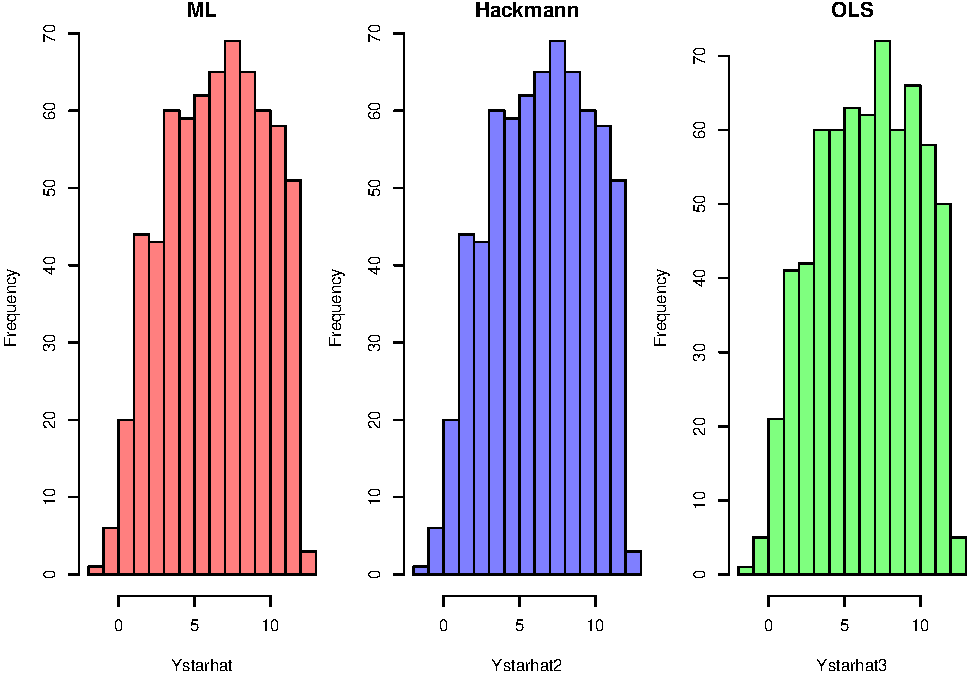
\includegraphics{assignment-5_files/figure-latex/unnamed-chunk-11-1.pdf}
As displayed above, the treatment effect before the intervention is
approximately stable around \(-0.2\). Except for 1929, no estimation is
significant at \(5\%\) or lower before 1937.

\begin{Shaded}
\begin{Highlighting}[]
\FunctionTok{linearHypothesis}\NormalTok{(m3, }\FunctionTok{c}\NormalTok{(}\StringTok{"treated:year::1925=0"}\NormalTok{, }\StringTok{"treated:year::1926=0"}\NormalTok{, }\StringTok{"treated:year::1927=0"}\NormalTok{, }\StringTok{"treated:year::1928=0"}\NormalTok{, }
                                  \StringTok{"treated:year::1929=0"}\NormalTok{, }\StringTok{"treated:year::1930=0"}\NormalTok{, }\StringTok{"treated:year::1931=0"}\NormalTok{, }\StringTok{"treated:year::1932=0"}\NormalTok{, }\StringTok{"treated:year::1933=0"}\NormalTok{, }\StringTok{"treated:year::1934=0"}\NormalTok{, }\StringTok{"treated:year::1935=0"}\NormalTok{))}
\end{Highlighting}
\end{Shaded}

\begin{verbatim}
## Warning: In vcov.fixest(model, complete = FALSE):
##  'complete' is not a valid argument of function vcov.fixest (fyi, some of
## its main arguments are 'vcov' and 'ssc').
\end{verbatim}

\begin{verbatim}
## Linear hypothesis test
## 
## Hypothesis:
## treated:year::1925 = 0
## treated:year::1926 = 0
## treated:year::1927 = 0
## treated:year::1928 = 0
## treated:year::1929 = 0
## treated:year::1930 = 0
## treated:year::1931 = 0
## treated:year::1932 = 0
## treated:year::1933 = 0
## treated:year::1934 = 0
## treated:year::1935 = 0
## 
## Model 1: restricted model
## Model 2: lnm_rate ~ treated * i(year, ref = 1936) | treated + year
## 
##   Df Chisq Pr(>Chisq)
## 1                    
## 2 11 9.337     0.5908
\end{verbatim}

The F test shows no joint significance, so we can assume common prior
trends. While this does not mean that parallel trends hold, these
results can be seen as suggestive towards the common trend assumption
necessary for difference-in-differences estimation.

After the medical intervention in 1937, we see a treatment effect
increasing in magnitude (i.e.~more negative) over the years until 1942,
with almost all coefficients significant even at the 0.1\(\%\)
confidence level. This is broadly in line with expectations as the
roll-out of innovative medicine likely evolves over the course of
several years and only coverges after multiple years. Furthermore, the
estimation in 1937 corresponds to our previous estimations validating
the results obtained above. After 1942, the treatment effect decreases
in magnitude, which might be due to the U.S. entering the WW2 such that
sulfa drugs supplies to the military were reduced thus lowering the
treatment intensity within U.S. states and increasing respective
mortality rates for scarlet fever.

\begin{enumerate}
\def\labelenumi{\roman{enumi})}
\setcounter{enumi}{5}
\tightlist
\item
  Argue at which level you need to cluster standard errors. Implement
  your suggested cluster-robust standard errors. Comment on your
  results.
\end{enumerate}

Follwoing the work of Abadie et al.~(2017) clustering should be viewed
as a design problem and necessitates that either the sampling process or
the treatment assignment is clustered. Due to lack of respective
information we disregard the former and only further discuss likely
clustering in the treatment assignment mechanism. Such clustering is
present if the assignment is correlated within clusters, but less so
across clusters (Abadie et al., 2017). For the treatment assignment
mechanism at hand, i.e.~the distribution of sulfa drugs, this is likely
the case for the state-level: the treatment intensity, i.e.~sulfa drug
adoption rate, is likely heterogeneous across states due to differences
in the quality of the local health care system (or due to religous
beliefs between member states and non-member states of the American
bible belt) and likely correlated across time within states, i.e.~across
observations within the suggested cluster. Therefore, all three models
(without state-fixed effects) are estimated again with cluster-robust
standard errors.

\begin{Shaded}
\begin{Highlighting}[]
\NormalTok{m1\_clustered }\OtherTok{\textless{}{-}} \FunctionTok{feols}\NormalTok{(lnm\_rate }\SpecialCharTok{\textasciitilde{}}\NormalTok{ D }\SpecialCharTok{|}\NormalTok{ treated }\SpecialCharTok{+}\NormalTok{ year, }\AttributeTok{data =} \FunctionTok{subset}\NormalTok{(data, data}\SpecialCharTok{$}\NormalTok{year }\SpecialCharTok{==} \DecValTok{1936}\SpecialCharTok{|}\NormalTok{ data}\SpecialCharTok{$}\NormalTok{year }\SpecialCharTok{==} \DecValTok{1937}\NormalTok{),}
            \AttributeTok{cluster =} \StringTok{\textquotesingle{}state\textquotesingle{}}\NormalTok{)}
\FunctionTok{summary}\NormalTok{(m1\_clustered)}
\end{Highlighting}
\end{Shaded}

\begin{verbatim}
## OLS estimation, Dep. Var.: lnm_rate
## Observations: 192 
## Fixed-effects: treated: 2,  year: 2
## Standard-errors: Clustered (state) 
##    Estimate Std. Error  t value   Pr(>|t|)    
## D -0.439008    0.08769 -5.00636 8.2331e-06 ***
## ---
## Signif. codes:  0 '***' 0.001 '**' 0.01 '*' 0.05 '.' 0.1 ' ' 1
## RMSE: 0.750306     Adj. R2: 0.848869
##                  Within R2: 0.020948
\end{verbatim}

\begin{Shaded}
\begin{Highlighting}[]
\NormalTok{m2\_clustered }\OtherTok{\textless{}{-}} \FunctionTok{feols}\NormalTok{(lnm\_rate }\SpecialCharTok{\textasciitilde{}}\NormalTok{ D }\SpecialCharTok{|}\NormalTok{ treated }\SpecialCharTok{+}\NormalTok{ year, data,}
            \AttributeTok{cluster =} \StringTok{\textquotesingle{}state\textquotesingle{}}\NormalTok{)}
\FunctionTok{summary}\NormalTok{(m2\_clustered)}
\end{Highlighting}
\end{Shaded}

\begin{verbatim}
## OLS estimation, Dep. Var.: lnm_rate
## Observations: 1,721 
## Fixed-effects: treated: 2,  year: 19
## Standard-errors: Clustered (state) 
##    Estimate Std. Error  t value  Pr(>|t|)    
## D -0.866724   0.041747 -20.7611 < 2.2e-16 ***
## ---
## Signif. codes:  0 '***' 0.001 '**' 0.01 '*' 0.05 '.' 0.1 ' ' 1
## RMSE: 0.605666     Adj. R2: 0.914713
##                  Within R2: 0.107824
\end{verbatim}

\begin{Shaded}
\begin{Highlighting}[]
\NormalTok{m3\_clustered }\OtherTok{\textless{}{-}} \FunctionTok{feols}\NormalTok{(lnm\_rate }\SpecialCharTok{\textasciitilde{}}\NormalTok{ treated}\SpecialCharTok{*}\FunctionTok{i}\NormalTok{(year, }\AttributeTok{ref =} \DecValTok{1936}\NormalTok{) }\SpecialCharTok{|}\NormalTok{ treated }\SpecialCharTok{+}\NormalTok{ year, data,}
 \AttributeTok{cluster =} \StringTok{\textquotesingle{}state\textquotesingle{}}\NormalTok{)}
\end{Highlighting}
\end{Shaded}

\begin{verbatim}
## Variables 'treated', 'year::1925' and 17 others have been removed because of collinearity (see $collin.var).
\end{verbatim}

\begin{Shaded}
\begin{Highlighting}[]
\FunctionTok{summary}\NormalTok{(m3\_clustered)}
\end{Highlighting}
\end{Shaded}

\begin{verbatim}
## OLS estimation, Dep. Var.: lnm_rate
## Observations: 1,721 
## Fixed-effects: treated: 2,  year: 19
## Standard-errors: Clustered (state) 
##                     Estimate Std. Error    t value   Pr(>|t|)    
## treated:year::1925 -0.135176   0.149351  -0.905092 3.7003e-01    
## treated:year::1926 -0.135567   0.150130  -0.903001 3.7113e-01    
## treated:year::1927 -0.222575   0.118074  -1.885041 6.5615e-02 .  
## treated:year::1928 -0.339383   0.101170  -3.354602 1.5791e-03 ** 
## treated:year::1929 -0.353351   0.130047  -2.717101 9.1901e-03 ** 
## treated:year::1930 -0.307318   0.123355  -2.491322 1.6314e-02 *  
## treated:year::1931 -0.314916   0.148894  -2.115031 3.9757e-02 *  
## treated:year::1932 -0.167430   0.123106  -1.360046 1.8030e-01    
## treated:year::1933 -0.144043   0.140443  -1.025634 3.1031e-01    
## treated:year::1934 -0.102580   0.116548  -0.880147 3.8326e-01    
## treated:year::1935 -0.069522   0.099514  -0.698608 4.8824e-01    
## treated:year::1937 -0.439008   0.087950  -4.991579 8.6551e-06 ***
## treated:year::1938 -0.704925   0.114943  -6.132850 1.6937e-07 ***
## treated:year::1939 -0.932996   0.124821  -7.474648 1.5647e-09 ***
## treated:year::1940 -1.139170   0.109368 -10.415908 8.4565e-14 ***
## treated:year::1941 -1.505930   0.134445 -11.201099 7.2654e-15 ***
## treated:year::1942 -1.384778   0.129455 -10.697020 3.4805e-14 ***
## treated:year::1943 -1.323763   0.133589  -9.909227 4.2949e-13 ***
## ... 19 variables were removed because of collinearity (treated, year::1925 and 17 others [full set in $collin.var])
## ---
## Signif. codes:  0 '***' 0.001 '**' 0.01 '*' 0.05 '.' 0.1 ' ' 1
## RMSE: 0.593665     Adj. R2: 0.917231
##                  Within R2: 0.142828
\end{verbatim}

In the first model, the standard errors decrease in comparison to the
previous estimation which is why the significance level at which the
identified treatment effect is significant increases to \(0.01\%\).
Essentially the same holds for the other estimations. Hence, our main
result of the signficant treatment effect of suilfa drugs on the
mortality of scarlet fever is robust against clustering adjustment.
However, the results of the prior trend analysis conducted above change
as more pre-trend coefficients become significant. A more detailed
analysis of this issue is left to subquestion (vii).

If one were to include state-fixed effects in the
difference-in-differences regressions, heterogeneity in the treatment
effect is required for clustering adjustment to be necessary because one
includes fixed effects at the level of the relevant clusters (Abadie et
al., 2017). To non-formally test for this heterogeneity, we interact
\(D_{gt}\) with states in the model specification of question (iv) and
test for the joint significance of the respective coefficients:

\begin{Shaded}
\begin{Highlighting}[]
\NormalTok{m\_states }\OtherTok{\textless{}{-}} \FunctionTok{feols}\NormalTok{(lnm\_rate }\SpecialCharTok{\textasciitilde{}}\NormalTok{ D }\SpecialCharTok{+}\NormalTok{ D}\SpecialCharTok{*}\NormalTok{state }\SpecialCharTok{|}\NormalTok{ state }\SpecialCharTok{+}\NormalTok{ treated }\SpecialCharTok{+}\NormalTok{ year, }\AttributeTok{data =}\NormalTok{ data, }\AttributeTok{se =} \StringTok{\textquotesingle{}standard\textquotesingle{}}\NormalTok{)}
\end{Highlighting}
\end{Shaded}

\begin{verbatim}
## Variables 'stateArizona', 'stateArkansas' and 45 others have been removed because of collinearity (see $collin.var).
\end{verbatim}

\begin{Shaded}
\begin{Highlighting}[]
\FunctionTok{summary}\NormalTok{(m\_states)}
\end{Highlighting}
\end{Shaded}

\begin{verbatim}
## OLS estimation, Dep. Var.: lnm_rate
## Observations: 1,721 
## Fixed-effects: state: 48,  treated: 2,  year: 19
## Standard-errors: IID 
##                        Estimate Std. Error   t value   Pr(>|t|)    
## D                     -1.183822   0.219140 -5.402122 7.5744e-08 ***
## D:stateArizona        -0.716911   0.313881 -2.284020 2.2500e-02 *  
## D:stateArkansas       -0.634731   0.304869 -2.081981 3.7502e-02 *  
## D:stateCalifornia     -0.450223   0.302896 -1.486396 1.3737e-01    
## D:stateColorado        0.407090   0.306152  1.329698 1.8381e-01    
## D:stateConnecticut    -0.333509   0.326597 -1.021166 3.0733e-01    
## D:stateDelaware        0.417789   0.302896  1.379317 1.6799e-01    
## D:stateFlorida        -0.392097   0.302896 -1.294496 1.9568e-01    
## D:stateGeorgia        -0.055693   0.306152 -0.181912 8.5567e-01    
## D:stateIdaho           0.830265   0.303815  2.732799 6.3487e-03 ** 
## D:stateIllinois        0.534617   0.302896  1.765020 7.7750e-02 .  
## D:stateIndiana         0.863162   0.302896  2.849702 4.4319e-03 ** 
## D:stateIowa            1.330784   0.302896  4.393540 1.1882e-05 ***
## D:stateKansas          1.096765   0.302896  3.620934 3.0266e-04 ***
## D:stateKentucky        0.656573   0.302896  2.167655 3.0331e-02 *  
## D:stateLouisiana      -0.517053   0.314900 -1.641959 1.0079e-01    
## D:stateMaine           0.337794   0.312989  1.079253 2.8064e-01    
## D:stateMaryland       -0.387721   0.302896 -1.280048 2.0071e-01    
## D:stateMassachusetts   0.182826   0.302896  0.603595 5.4620e-01    
## D:stateMichigan        0.702168   0.302896  2.318185 2.0564e-02 *  
## D:stateMinnesota       0.529232   0.302896  1.747243 8.0786e-02 .  
## D:stateMississippi    -0.388098   0.302896 -1.281293 2.0028e-01    
## D:stateMissouri        0.540234   0.304869  1.772021 7.6581e-02 .  
## D:stateMontana         1.008002   0.302896  3.327888 8.9485e-04 ***
## D:stateNebraska        1.293606   0.302896  4.270800 2.0619e-05 ***
## D:stateNevada          0.850406   0.380653  2.234071 2.5616e-02 *  
## D:stateNew Hampshire   0.525746   0.302896  1.735735 8.2802e-02 .  
## D:stateNew Jersey     -0.102548   0.302896 -0.338559 7.3499e-01    
## D:stateNew Mexico     -0.263847   0.307649 -0.857624 3.9123e-01    
## D:stateNew York       -0.114624   0.302896 -0.378426 7.0516e-01    
## D:stateNorth Carolina  0.092499   0.302896  0.305382 7.6011e-01    
## D:stateNorth Dakota    0.916629   0.312990  2.928621 3.4527e-03 ** 
## D:stateOhio            0.546121   0.302896  1.803000 7.1576e-02 .  
## D:stateOklahoma        0.204982   0.306152  0.669543 5.0325e-01    
## D:stateOregon          0.497977   0.302896  1.644056 1.0036e-01    
## D:statePennsylvania    0.350548   0.302896  1.157322 2.4731e-01    
## D:stateRhode Island    0.194773   0.312988  0.622300 5.3383e-01    
## D:stateSouth Carolina -0.254767   0.312989 -0.813981 4.1578e-01    
## D:stateSouth Dakota    0.675414   0.314163  2.149883 3.1713e-02 *  
## D:stateTennessee       0.086348   0.304869  0.283230 7.7704e-01    
## D:stateTexas          -0.415892   0.317439 -1.310145 1.9033e-01    
## D:stateUtah            0.989471   0.312991  3.161337 1.5998e-03 ** 
## D:stateVermont         0.229843   0.302896  0.758818 4.4807e-01    
## D:stateVirginia       -0.073795   0.302896 -0.243633 8.0755e-01    
## D:stateWashington      0.410533   0.302896  1.355362 1.7549e-01    
## D:stateWest Virginia   0.791172   0.302896  2.612028 9.0846e-03 ** 
## D:stateWisconsin       1.044326   0.302896  3.447808 5.7974e-04 ***
## D:stateWyoming         1.323630   0.312991  4.228969 2.4800e-05 ***
## ... 47 variables were removed because of collinearity (stateArizona, stateArkansas and 45 others [full set in $collin.var])
## ---
## Signif. codes:  0 '***' 0.001 '**' 0.01 '*' 0.05 '.' 0.1 ' ' 1
## RMSE: 0.490989     Adj. R2: 0.940671
##                  Within R2: 0.269909
\end{verbatim}

\begin{Shaded}
\begin{Highlighting}[]
\FunctionTok{linearHypothesis}\NormalTok{(m\_states, }\FunctionTok{c}\NormalTok{(}\StringTok{"D:stateArizona=0"}\NormalTok{,}\StringTok{"D:stateArkansas=0"}\NormalTok{,}\StringTok{"D:stateCalifornia=0"}\NormalTok{,}\StringTok{"D:stateColorado=0"}\NormalTok{,}\StringTok{"D:stateConnecticut=0"}\NormalTok{,}\StringTok{"D:stateDelaware=0"}\NormalTok{,}\StringTok{"D:stateFlorida=0"}\NormalTok{,}\StringTok{"D:stateGeorgia=0"}\NormalTok{,}\StringTok{"D:stateIdaho=0"}\NormalTok{,}\StringTok{"D:stateIllinois=0"}\NormalTok{,}\StringTok{"D:stateIndiana=0"}\NormalTok{,}\StringTok{"D:stateIowa=0"}\NormalTok{,}\StringTok{"D:stateKansas=0"}\NormalTok{,}\StringTok{"D:stateKentucky=0"}\NormalTok{,}\StringTok{"D:stateLouisiana=0"}\NormalTok{,}\StringTok{"D:stateMaine=0"}\NormalTok{,}\StringTok{"D:stateMaryland=0"}\NormalTok{,}\StringTok{"D:stateMassachusetts=0"}\NormalTok{,}\StringTok{"D:stateMichigan=0"}\NormalTok{,}\StringTok{"D:stateMinnesota=0"}\NormalTok{,}\StringTok{"D:stateMississippi=0"}\NormalTok{,}\StringTok{"D:stateMissouri=0"}\NormalTok{,}\StringTok{"D:stateMontana=0"}\NormalTok{,}\StringTok{"D:stateNebraska=0"}\NormalTok{,}\StringTok{"D:stateNevada=0"}\NormalTok{,}\StringTok{"D:stateNew Hampshire=0"}\NormalTok{,}\StringTok{"D:stateNew Jersey=0"}\NormalTok{,}\StringTok{"D:stateNew Mexico=0"}\NormalTok{,}\StringTok{"D:stateNew York=0"}\NormalTok{,}\StringTok{"D:stateNorth Carolina=0"}\NormalTok{,}\StringTok{"D:stateNorth Dakota=0"}\NormalTok{,}\StringTok{"D:stateOhio=0"}\NormalTok{,}\StringTok{"D:stateOklahoma=0"}\NormalTok{,}\StringTok{"D:stateOregon=0"}\NormalTok{,}\StringTok{"D:statePennsylvania=0"}\NormalTok{,}\StringTok{"D:stateRhode Island=0"}\NormalTok{,}\StringTok{"D:stateSouth Carolina=0"}\NormalTok{,}\StringTok{"D:stateSouth Dakota=0"}\NormalTok{,}\StringTok{"D:stateTennessee=0"}\NormalTok{,}\StringTok{"D:stateTexas=0"}\NormalTok{,}\StringTok{"D:stateUtah=0"}\NormalTok{,}\StringTok{"D:stateVermont=0"}\NormalTok{,}\StringTok{"D:stateVirginia=0"}\NormalTok{,}\StringTok{"D:stateWashington=0"}\NormalTok{,}\StringTok{"D:stateWest Virginia=0"}\NormalTok{,}\StringTok{"D:stateWisconsin=0"}\NormalTok{,}\StringTok{"D:stateWyoming=0"}\NormalTok{))}
\end{Highlighting}
\end{Shaded}

\begin{verbatim}
## Warning: In vcov.fixest(model, complete = FALSE):
##  'complete' is not a valid argument of function vcov.fixest (fyi, some of
## its main arguments are 'vcov' and 'ssc').
\end{verbatim}

\begin{verbatim}
## Linear hypothesis test
## 
## Hypothesis:
## D:stateArizona = 0
## D:stateArkansas = 0
## D:stateCalifornia = 0
## D:stateColorado = 0
## D:stateConnecticut = 0
## D:stateDelaware = 0
## D:stateFlorida = 0
## D:stateGeorgia = 0
## D:stateIdaho = 0
## D:stateIllinois = 0
## D:stateIndiana = 0
## D:stateIowa = 0
## D:stateKansas = 0
## D:stateKentucky = 0
## D:stateLouisiana = 0
## D:stateMaine = 0
## D:stateMaryland = 0
## D:stateMassachusetts = 0
## D:stateMichigan = 0
## D:stateMinnesota = 0
## D:stateMississippi = 0
## D:stateMissouri = 0
## D:stateMontana = 0
## D:stateNebraska = 0
## D:stateNevada = 0
## D:stateNew Hampshire = 0
## D:stateNew Jersey = 0
## D:stateNew Mexico = 0
## D:stateNew York = 0
## D:stateNorth Carolina = 0
## D:stateNorth Dakota = 0
## D:stateOhio = 0
## D:stateOklahoma = 0
## D:stateOregon = 0
## D:statePennsylvania = 0
## D:stateRhode Island = 0
## D:stateSouth Carolina = 0
## D:stateSouth Dakota = 0
## D:stateTennessee = 0
## D:stateTexas = 0
## D:stateUtah = 0
## D:stateVermont = 0
## D:stateVirginia = 0
## D:stateWashington = 0
## D:stateWest Virginia = 0
## D:stateWisconsin = 0
## D:stateWyoming = 0
## 
## Model 1: restricted model
## Model 2: lnm_rate ~ D + D * state | state + treated + year
## 
##   Df  Chisq Pr(>Chisq)    
## 1                         
## 2 47 299.38  < 2.2e-16 ***
## ---
## Signif. codes:  0 '***' 0.001 '**' 0.01 '*' 0.05 '.' 0.1 ' ' 1
\end{verbatim}

Based on the F-test reported above the interaction-coefficients are
jointly significanr such that we find evidence for heterogeneous
treatment effects here. In this case Abadie et al.~(2017) suggest that a
clustering adjustment is also necessary, if one were to include fixed
effects at the level of the state-cluster in the regression
specification. The analysis adopted here is, however, of rather
superficial nature such that more rigirous testing of heterogeneity in
treatment effects would be necessary at this point.

\begin{enumerate}
\def\labelenumi{\roman{enumi})}
\setcounter{enumi}{6}
\tightlist
\item
  Do a test of whether the prior trends differ between the treated and
  control groups. What do you conclude?
\end{enumerate}

To test whether the prior trends differ between the treated and control
groups, we run a F-test of the joint significant of all pre-trend
coefficients estimated by the model specified in (v) with clustered
standard erros, i.e.~\(\hat{\delta}_{t-\tau}\) for which \(t-\tau<-1\):

\begin{Shaded}
\begin{Highlighting}[]
\FunctionTok{linearHypothesis}\NormalTok{(m3\_clustered, }\FunctionTok{c}\NormalTok{(}\StringTok{"treated:year::1925=0"}\NormalTok{, }\StringTok{"treated:year::1926=0"}\NormalTok{, }\StringTok{"treated:year::1927=0"}\NormalTok{, }\StringTok{"treated:year::1928=0"}\NormalTok{, }
                                  \StringTok{"treated:year::1929=0"}\NormalTok{, }\StringTok{"treated:year::1930=0"}\NormalTok{, }\StringTok{"treated:year::1931=0"}\NormalTok{, }\StringTok{"treated:year::1932=0"}\NormalTok{, }\StringTok{"treated:year::1933=0"}\NormalTok{, }\StringTok{"treated:year::1934=0"}\NormalTok{, }\StringTok{"treated:year::1935=0"}\NormalTok{))}
\end{Highlighting}
\end{Shaded}

\begin{verbatim}
## Warning: In vcov.fixest(model, complete = FALSE):
##  'complete' is not a valid argument of function vcov.fixest (fyi, some of
## its main arguments are 'vcov' and 'ssc').
\end{verbatim}

\begin{verbatim}
## Linear hypothesis test
## 
## Hypothesis:
## treated:year::1925 = 0
## treated:year::1926 = 0
## treated:year::1927 = 0
## treated:year::1928 = 0
## treated:year::1929 = 0
## treated:year::1930 = 0
## treated:year::1931 = 0
## treated:year::1932 = 0
## treated:year::1933 = 0
## treated:year::1934 = 0
## treated:year::1935 = 0
## 
## Model 1: restricted model
## Model 2: lnm_rate ~ treated * i(year, ref = 1936) | treated + year
## 
##   Df  Chisq Pr(>Chisq)    
## 1                         
## 2 11 38.142  7.404e-05 ***
## ---
## Signif. codes:  0 '***' 0.001 '**' 0.01 '*' 0.05 '.' 0.1 ' ' 1
\end{verbatim}

After adjusting the standard errors for clustering, the estimated prior
trend coefficients, i.e.~treatment effect coefficients before the
intervention, are jointly significant indicating violations of common
prior trends. However, with prior trends we are less concerned with
significance than with the size of the estimations. After all, in
comparison to the treatment effect during treated years, the estimations
for the pre-treatment years are substantially lower.

Moreover, it does not seem completely unlikely that the introduction of
sulfa drugs has been timely correlated with preceding advancements in
medication of diseases which can also be medicated with sulfa drugs. If
this were the case, one would not be surprised pre-treatment treatment
effect coefficients shortly before the actual intervention to be
significant.

Furthermore, equal prior trends do not necessarily imply that parallel
trends over the treatment period hold, and one might as well argue
(e.g.~based on additional data) that the development of mortality rates
across diseases converged overall within the considered treatment
period.

\hypertarget{references}{%
\section{References}\label{references}}

Abadie, A., Athey, S., Imbens, G. W., \& Wooldridge, J. (2017). When
should you adjust standard errors for clustering? (No.~w24003). National
Bureau of Economic Research.

De Chaisemartin, C., \& d'Haultfoeuille, X. (2020). Two-way fixed
effects estimators with heterogeneous treatment effects. American
Economic Review, 110(9), 2964-96.

Ozsoy, S. M., Rasteh, M., \& Yönder, E. (2020). Understanding drought
shocks: Bank financial stability and loan performance. Working Paper.

\end{document}
